\section{Base Theory and Concepts About Graphics}

\subsection{Image Representation}

\begin{frame}{Light, pixels and pictures}
  \begin{minipage}{0.75\textwidth}
  \begin{itemize}
  \item Pictures are {\bf representations of light emissions}
  \item Analog representations are spatially {\bf continuous}:
    \begin{itemize}
    \item With an {\bf infinite} number of elements
    \item Example: photosensitive paper
    \end{itemize}
  \item Digital representations are spatially {\bf quantified}:
    \begin{itemize}
    \item With a {\bf finite} number of elements
    \item Example: discrete LED-based display
    \end{itemize}
  \item Producing a digital representation is called \textbf{quantization}
    \begin{itemize}
    \item Reduction of information from the continuous world
    \item Quantization requires a {\bf base element unit} or quantum
    \item This quantum is called picture element or {\bf pixel}
    \item Quantization is also called \textbf{sampling} in this context
    \end{itemize}
  \end{itemize}
  \end{minipage}%
  \begin{minipage}{0.25\textwidth}
  \includegraphics[width=\textwidth]{slides/graphics-theory-image/ccc-rocket.jpg}
  \end{minipage}
\end{frame}

\begin{frame}{Light, pixels and pictures}
  \begin{itemize}
  \item \textbf{Pictures} (or frames) are bi-dimensional ordered ensembles of pixels:
    \begin{itemize}
    \item Frames have \textbf{dimensions} (or size): \textbf{width} (horizontal) and \textbf{height} (vertical)
    \item The aspect ratio is the \textbf{width:height} ratio (e.g. 16:9, 4:3)
    \item Pixels are located with a \textbf{position}: \textbf{(x,y)}
    \item The dimension and position unit is the number of pixels
    \end{itemize}
  \item Quantified pixels have a \textbf{spatial density} or spatial resolution:\\
    \begin{itemize}
    \item \textit{How many pixels are found in \(n\) inches?}
    \item The usual pixel resolution unit is the \textbf{dot per inch} (DPI)
    \item Vertical and horizontal spatial densities are usually not distinguished\\
      \textit{pixels are assumed to have a square shape most of the time}
    \end{itemize}
  \end{itemize}

\end{frame}

\begin{frame}{Light, pixels and pictures (illustrated)}
  \begin{minipage}[b]{0.45\textwidth}
    \centering
    \includegraphics[width=\textwidth]{slides/graphics-theory-image/first-photo.jpg}
    \textit{\small View from the Window at Le Gras picture}
  \end{minipage}
  \hfill
  \begin{minipage}[b]{0.45\textwidth}
    \centering
    \includegraphics[width=\textwidth]{slides/graphics-theory-image/dot-matrix-display.jpg}
    \textit{\small A monochrome dot-matrix display}
  \end{minipage}

  \vspace{1em}

  \begin{minipage}[b]{0.45\textwidth}
    \centering
    \textbf{Analog representation},\\ on a metal plate
  \end{minipage}
  \hfill
  \begin{minipage}[b]{0.45\textwidth}
    \centering
    \textbf{Digital representation},\\ on a LED display
  \end{minipage}
\end{frame}

\begin{frame}{Sampling and frequency domain}
  \begin{itemize}
  \item Pixels are quantized/sampled representations of a \textbf{spatial domain}
  \item The initial (continuous) domain has a corresponding \textbf{frequency spectrum}\\
    \textit{high frequencies provide details in pictures}
  \item A 2D \textbf{Fourier transform} translates from spatial \((x,y)\) to frequency \((u,v)\) domain
\[
F(u,v) = \int_{-\infty}^{+\infty} \int_{-\infty}^{+\infty} f(x,y)e^{-j2\pi(ux+vy)}dxdy
\]
  \item The transform decomposes the domain in \textbf{periodic patterns}
  \item Adapted for discrete signals as \textbf{Discrete Fourier Transform}
  \item Implemented with optimized algorithms as \textbf{Fast Fourier Transform} (FFT)
  \item \textbf{Frequency domain analysis} is very useful for signal processing\\
    \textit{used at the roots of image compression}
  \end{itemize}
\end{frame}

\begin{frame}{Sampling and frequency domain (illustrated)}
  \begin{center}
  \begin{minipage}[b]{0.45\textwidth}
    \centering
    \includegraphics[width=\textwidth]{slides/graphics-theory-image/bricks.jpg}\\
    \textit{\small A wall of bricks represented in the spatial domain}
  \end{minipage}
  \hfill
  \begin{minipage}[b]{0.45\textwidth}
    \centering
    \includegraphics[width=\textwidth]{slides/graphics-theory-image/bricks-fft.jpg}\\
    \textit{\small The wall of bricks represented in the frequency domain}
  \end{minipage}

  \end{center}
\end{frame}

\begin{frame}{Sampling and frequency domain (illustrated)}
  \begin{minipage}[b]{0.45\textwidth}
    \centering
    \includegraphics[width=\textwidth]{slides/graphics-theory-image/bricks-rotation.jpg}\\
    \textit{\small A wall of bricks rotated \(45^{\circ}\) represented in the spatial domain}
  \end{minipage}
  \hfill
  \begin{minipage}[b]{0.45\textwidth}
    \centering
    \includegraphics[width=\textwidth]{slides/graphics-theory-image/bricks-fft-rotation.jpg}\\
    \textit{\small The wall of bricks rotated \(45^{\circ}\) represented in the frequency domain}
  \end{minipage}
\end{frame}

\begin{frame}{Sampling and aliasing}
  \begin{itemize}
  \item The spatial domain is quantized with a bi-dimensional \textbf{sampling resolution}
  \item Matching \textbf{sampling frequencies} exist, for each axis: \((u_s,v_s)\)
  \item They \textbf{limit the frequencies} that can be sampled from the initial domain
  \item The \textbf{Shannon-Nyquist theorem} provides a sufficient condition for \((u_s,v_s)\):
\[
u_s > 2 \times u_{max}, ~v_s > 2 \times v_{max}
\]
  \item Frequencies such that \(u \geq \frac{u_s}{2}\) and \(v \geq \frac{v_s}{2}\) are \textbf{not correctly sampled}
  \item Can result in \textbf{incorrect frequencies} being introduced: \textbf{Moiré pattern} in 2D
  \end{itemize}

  \begin{center}
  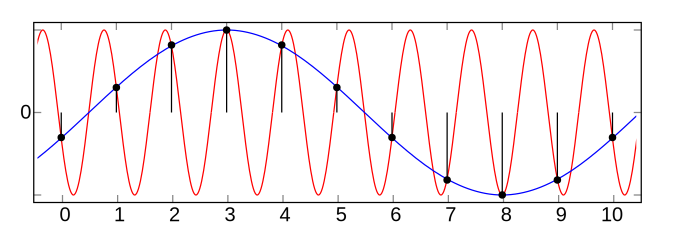
\includegraphics[width=0.35\textwidth]{slides/graphics-theory-image/aliasing-1d.pdf}\\
  \textit{\small Aliasing example in a uni-dimensional domain}
  \end{center}
\end{frame}

\begin{frame}{Sampling and aliasing (illustrated)}
  \begin{minipage}[b]{0.29\textwidth}
    \centering
    \includegraphics[width=\textwidth]{slides/graphics-theory-image/bricks-rich.jpg}\\
    \textit{\small Another wall of bricks}
  \end{minipage}
  \hfill
  \begin{minipage}[b]{0.29\textwidth}
    \centering
    \includegraphics[width=\textwidth]{slides/graphics-theory-image/bricks-alias.jpg}\\
    \textit{\small Moiré on the bricks}
  \end{minipage}
  \hfill
  \begin{minipage}[b]{0.29\textwidth}
    \centering
    \includegraphics[width=\textwidth]{slides/graphics-theory-image/moire.jpg}\\
    \textit{\small Moiré on the garage door}
  \end{minipage}
\end{frame}
